\subsection{Dati città}
\label{sec:dati_città}
Dopo aver selezionato la città desiderata, verrà visualizzata la schermata dei dati della città:
\begin{figure}[H]
    \centering
    \includegraphics[width=1\textwidth]{../../img/dati_città.png}
    \caption{Schermata Dati città}
\end{figure}

Nella schermata è possibile vedere:
\begin{itemize}
    \item Il nome della città selezionata. 
    \item La nazione a cui appartiene la città selezionata.
    \item Le coordinate geografiche della città selezionata.
    \item La media dei punteggi per ogni parametro climatico rilevato.
    \item Il numero di rilevazioni effettuate per ogni parametro climatico.
    \item Gli eventuali commenti inseriti dagli operatori per ogni parametro climatico.
\end{itemize}

Per sapere a quali fasce appartengono i punteggi visualizzati, fare riferimento alla sezione \ref{sec:legenda_punteggi} del presente manuale oppure fare click sul punteggio
desiderato per visualizzare la relativa legenda:
\begin{figure}[H]
    \centering
    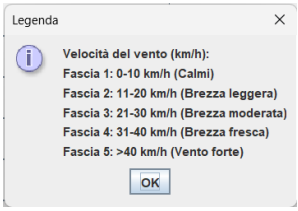
\includegraphics[width=0.7\textwidth]{../../img/esempio_legenda.png}
    \caption{Esempio di legenda}
\end{figure}

Se sono presenti molti commenti per un singolo parametro e non sono interamente visibili, è possibile visualizzarli tutti cliccando sul commento desiderato:
\begin{figure}[H]
    \centering
    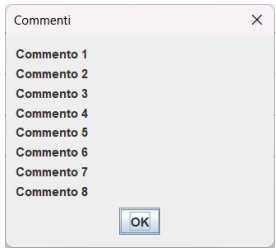
\includegraphics[width=0.7\textwidth]{../../img/esempio_commenti.png}
    \caption{Esempio di commenti}
\end{figure}